\documentclass[t,handout]{beamer}   % overlays

\usetheme{Madrid}
\usecolortheme{beaver}
\usepackage{tikz}
\usetikzlibrary{fit,arrows,calc,positioning}

%\usepackage{emerald} 
\usepackage[T1]{fontenc} 


\usepackage{graphicx}
\usepackage{epsfig}
\usepackage{psfrag}
\usepackage[english]{babel}
\usepackage{listings}
\usepackage{courier}
\usepackage{color}
\usepackage[backend=bibtex,style=ieee]{biblatex}

\lstset{
	language=Ruby,
	basicstyle=\footnotesize\ttfamily\color{black},
	commentstyle = \footnotesize\ttfamily\color{red},
	keywordstyle=\footnotesize\ttfamily\color{blue},
	stringstyle=\footnotesize\ttfamily\color{black},
%	columns=fixed,
%	numbers=left,    
	numberstyle=\tiny,
	stepnumber=1,
	numbersep=5pt,
	tabsize=1,
	extendedchars=true,
	breaklines=true,            
	frame=b,         
	showspaces=false,
	showtabs=true,
	xleftmargin=6pt,
	framexleftmargin=6pt,
	framexrightmargin=2pt,
	framexbottommargin=4pt,
	showstringspaces=false      
}

\lstloadlanguages{
         Ruby,HTML
}

\graphicspath{ {./images/} }  % Figures path - used in graphicx

%\selectcolormodel{cmyk}

\mode<presentation>

\renewcommand*{\bibfont}{\tiny}

\newcommand{\dred}{darkred!90!black}
\newcommand{\written}{\ECFJD\textcolor{cyan!50!white}}
\newcommand{\hlight}{\textcolor{\dred}}
\newcommand{\Ex}{\textcolor{\dred}{Ex. }}

% remove navigation symbols in full screen mode
\setbeamertemplate{navigation symbols}{}  
\setbeamertemplate{blocks}[rounded][shadow=false]
\setbeamertemplate{itemize items}[default]
\setbeamertemplate{enumerate items}[default]
\setbeamertemplate{sections/subsections in toc}[circle]
\setbeamercolor{note page}{fg=black}

\setbeamercolor{title}{fg=\dred}
\setbeamercolor{frametitle}{fg=white}
\setbeamercolor{frametitle}{bg=\dred}
\setbeamercolor{structure}{fg=black,bg=white}
\setbeamercolor{background canvas}{bg=white,fg=black}
\setbeamercolor{normal text}{fg=black,bg=white}
\setbeamercolor{item}{fg=red!80!black,bg=white!}
\addtobeamertemplate{block begin}{\setbeamercolor{block title}{fg=white,bg=\dred}
\setbeamercolor{block body}{fg=\dyellow,bg=gray!50!black}}{}



\addbibresource{bib/aws.bib}

\title[]
{(E)EMI in Computing Systems}

\author[Heileman, Valbuena, Piro-Rael] % (optional, use only with lots of authors)
{\bf Gregory L. Heileman \ \ \ \ Luis Valbuena \ \ \ \ Ricardo Piro-Rael}

\institute[]
{Informatics Laboratory \\
Department of Electrical \& Computer Engineering \\
University of New Mexico}

\date[June 10, 2015]

\begin{document}

\begin{frame}
  \titlepage
\end{frame}
\note{Talk for 10 minutes} 

\addtobeamertemplate{frametitle}{}{%
\begin{tikzpicture}[remember picture,overlay]
\node[anchor=north east,yshift=-1pt] at (current page.north east) {
\includegraphics[width = 1in]{UNMLogo.png}};
\end{tikzpicture}}

%%%%%%%%%%%%%%%%%%%%%%%%%%%%%%%%%%%%%%%%%%%%%%%%%%%%%%

\section*{Outline}

\begin{frame}  \frametitle{Outline}  
	\tableofcontents
\end{frame}

\section{Introduction}

\begin{frame}{Introduction}
\begin{itemize}
\vspace*{-0.2in}
 \item The Informatics Laboratory, located in the Department of Electrical \& Computer Engineering at the University of New Mexico, is a multi-disciplinary research group focused on ``informatics.''~\\~\\
 \pause
 \item Informatics is concerned with the science around information processing and analytics, and the engineering of information systems.~\\~\\
 \pause
 \item Our research has focused primarily on the areas of information security, assured information sharing in complex distributed systems,  information architectures, and data science (big data, information analytics, semantic representations, data visualization).~\\~\\
 \pause
 \item We have stood up a private cloud computing infrastructure in the lab for experimentation purposes.
 \end{itemize}
\end{frame}

\begin{frame}{Introduction}
%\begin{itemize}
% \item As a part of this research effort, we will investigate how EM radiation may lead to unintended state changes in the memory and combinatorial logic circuits associated with a computing system, and how these may lead to software errors, and changes in computing system behavior.~\\~\\
% \pause
% \item If these faults can be injected in any sort of predictable fashion, there are numerous system security exploits that might be enabled.~\\~\\
% \pause
% \item Thus, we will further explore the various ways in which these state changes may be leveraged in order to compromise  computing systems.  \pause How do these effects translate up the stack of the hardware/software machine hierarchy?
% \end{itemize}
\end{frame}

\section{Background}

\begin{frame}{Background}
%Early instances of EMI-based fault injection:
% \begin{itemize}
%    \item Aerospace hardware affected by solar wind and cosmic rays.
%    \pause
%    \item Residues of radioactive material that release $\alpha$ particles~\cite{Sorcerer_Fault_Attacks}.
%    \end{itemize}~\\
% \pause
%These can ``flip'' bits in the circuits of an IC, thereby affecting the combinatorial logic circuits associated with the computing system.
\end{frame}

\begin{frame}{Background}
 	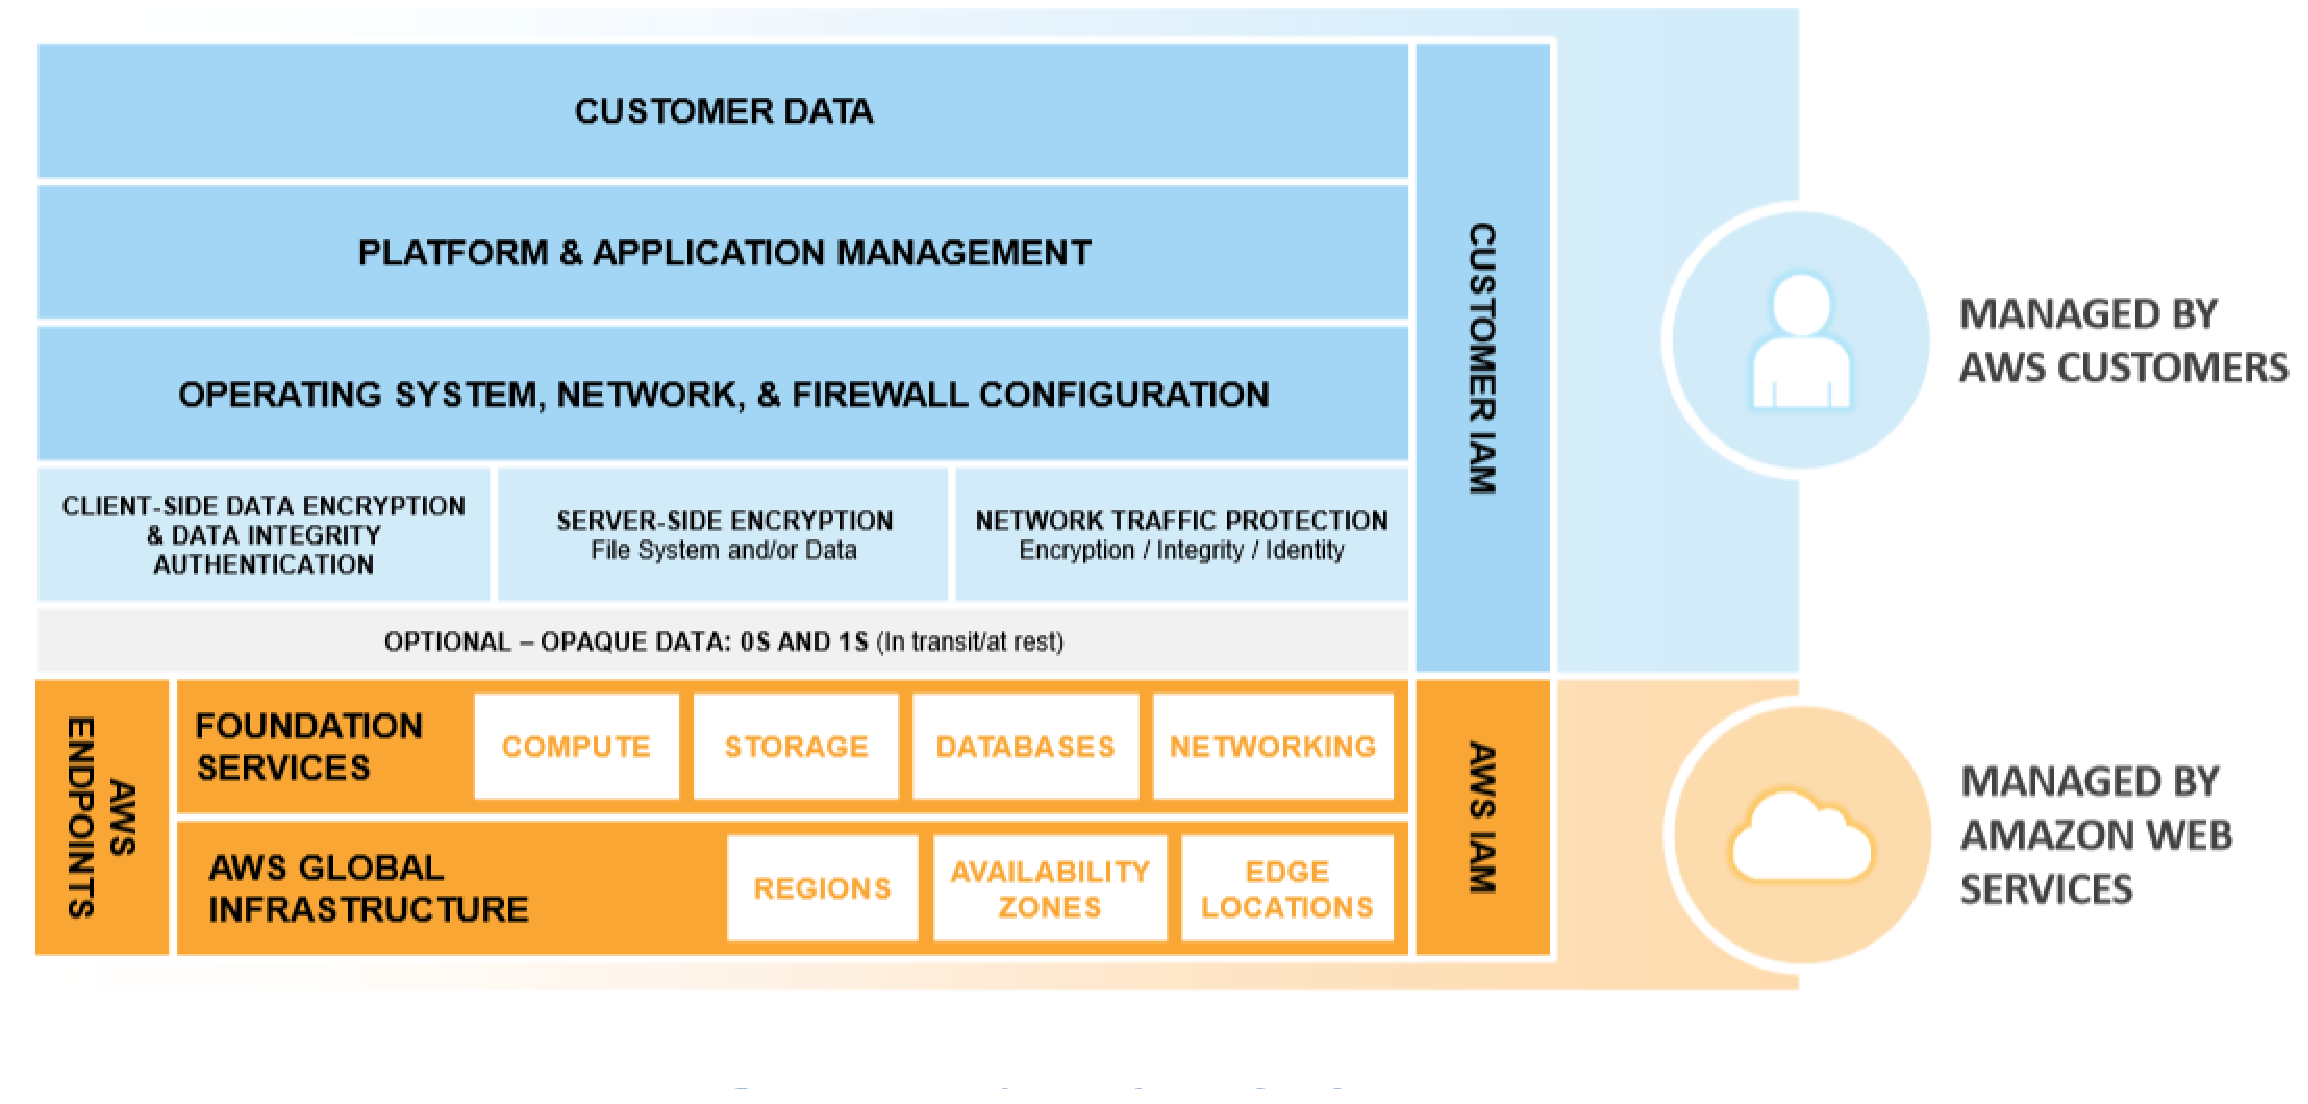
\includegraphics[width=\textwidth]{442-mod.pdf} \\~\\~\\
 	{\tiny Extracted from content provided by Amazon Web Services\cite{Aws:15}.}
\end{frame}

\begin{frame}{Background}
 	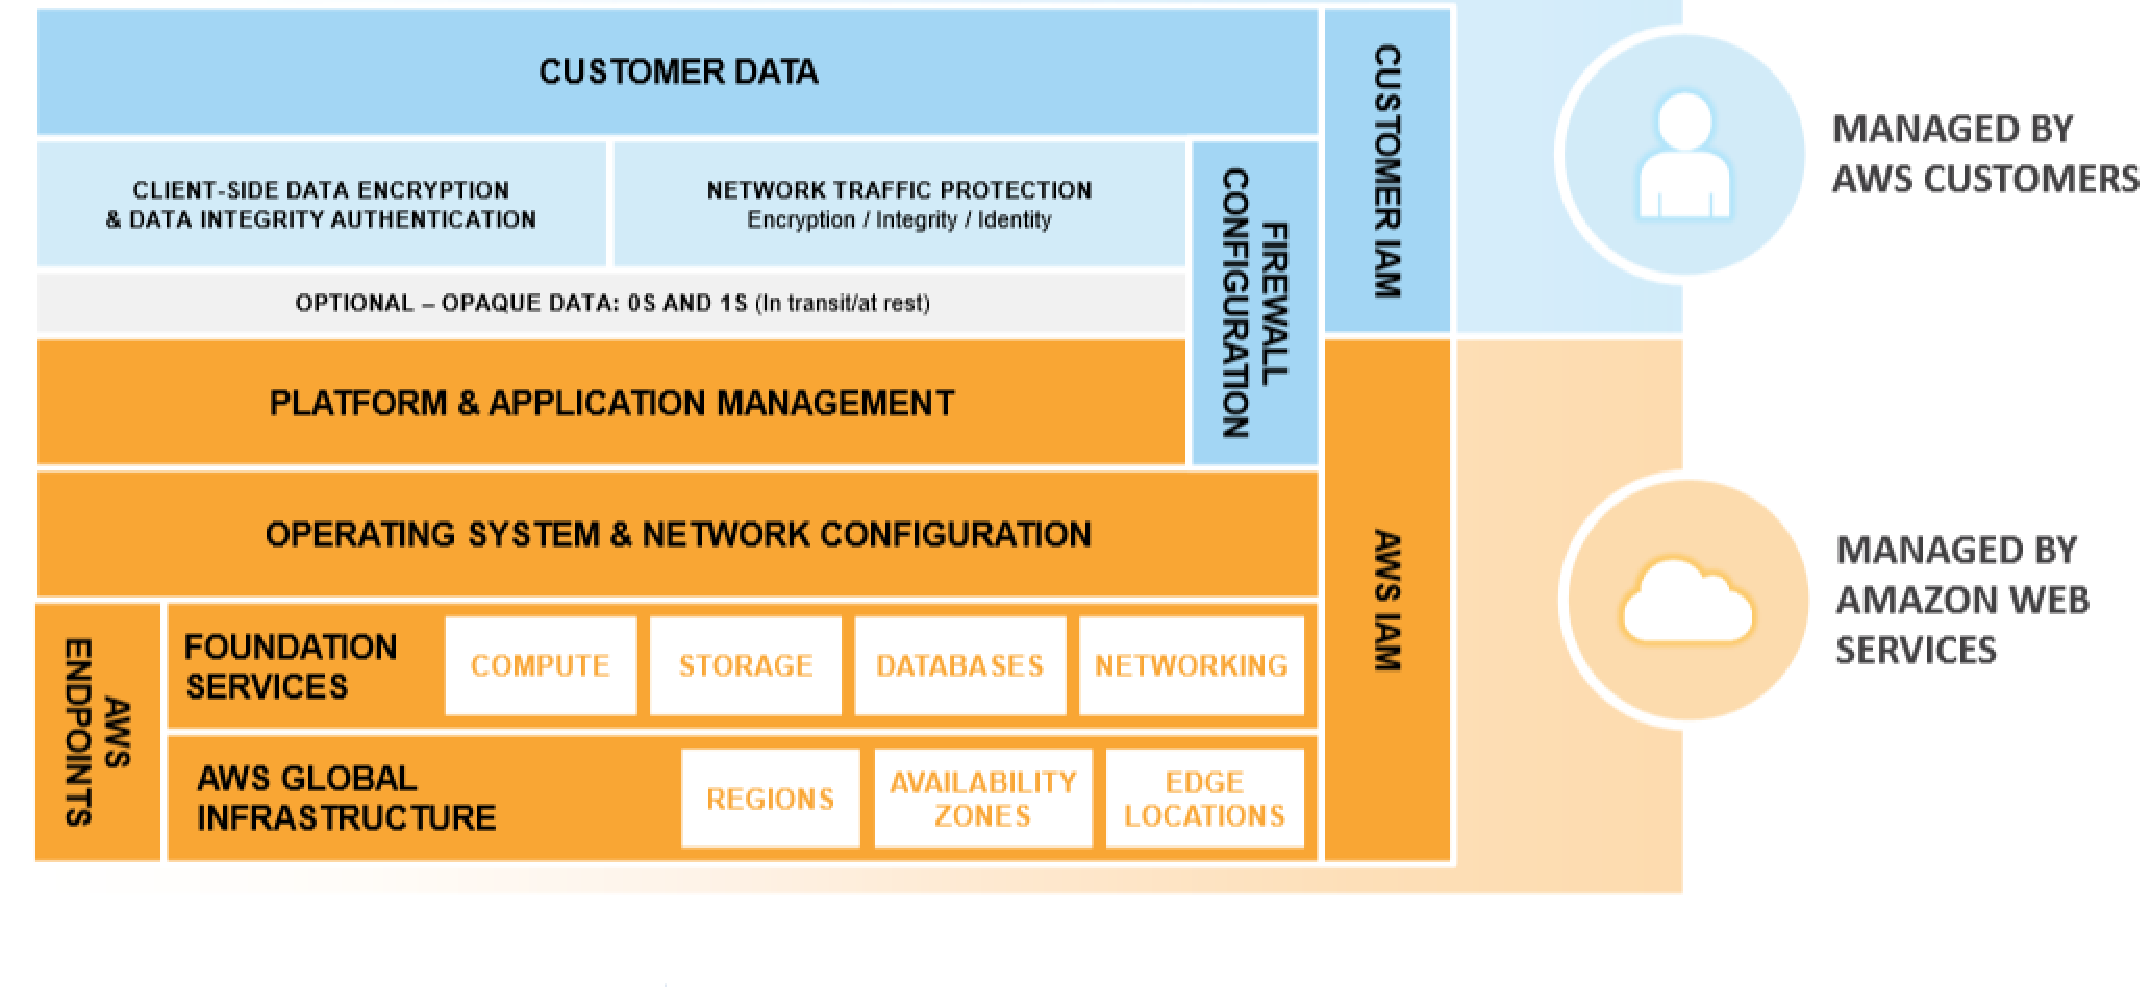
\includegraphics[width=\textwidth]{445-mod.pdf} \\~\\~\\
 	{\tiny Extracted from content provided by Amazon Web Services\cite{Aws:15}.}
\end{frame}

\begin{frame}{Background}
 	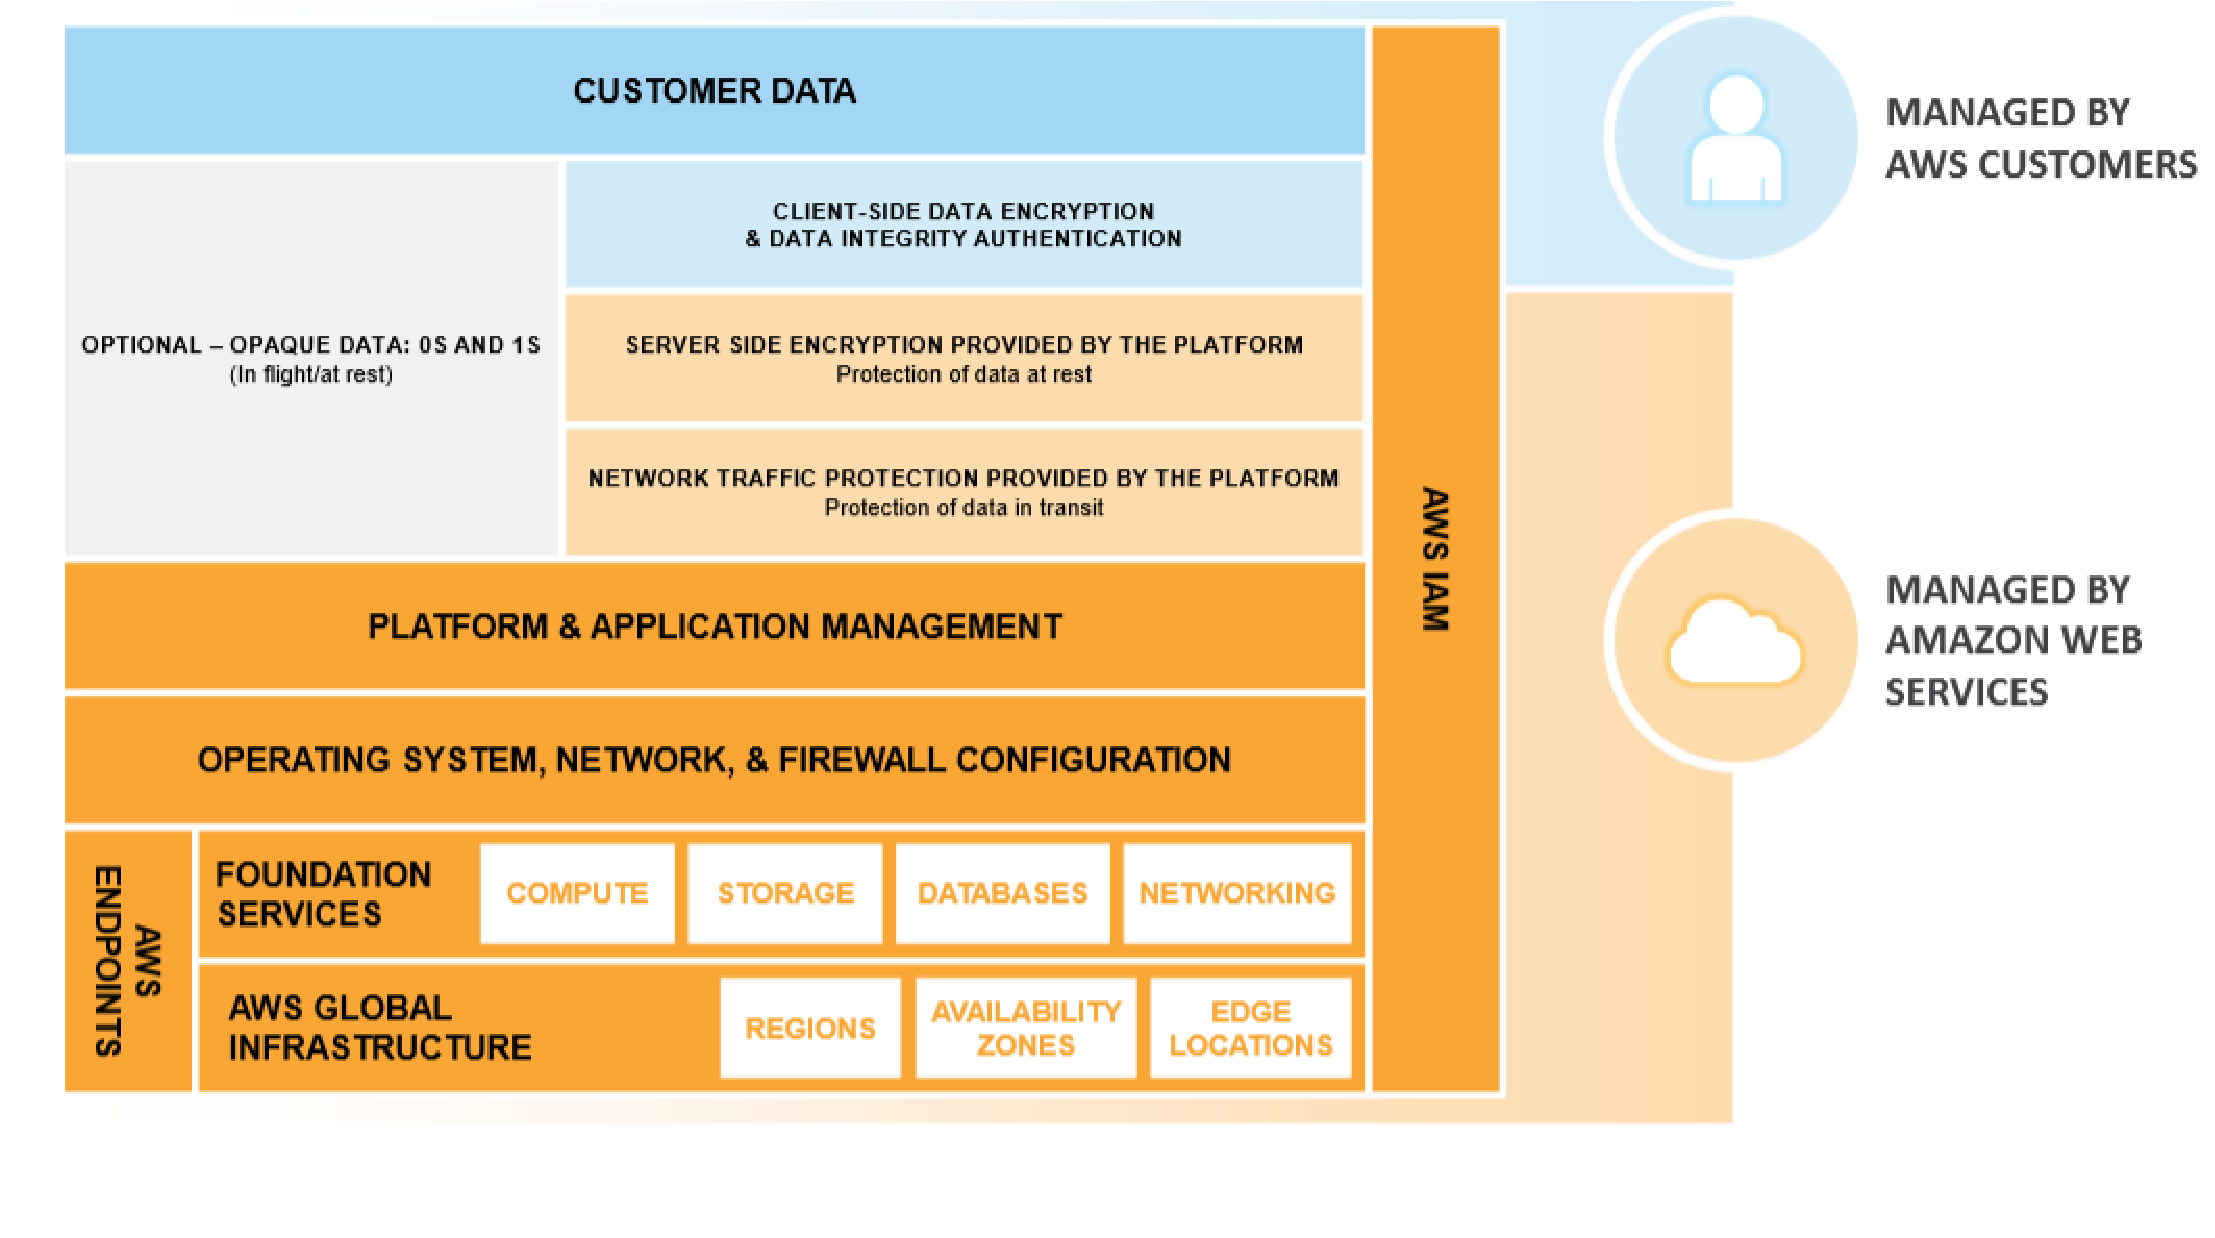
\includegraphics[width=\textwidth]{448-mod.pdf} \\
 	{\tiny Extracted from content provided by Amazon Web Services\cite{Aws:15}.}
\end{frame}

\begin{frame}[allowframebreaks]{Bibliography}
 	\def\newblock{}	
	\printbibliography
\end{frame}

\end{document}
